\chapter{Experimente}\label{ch:Experimente}

\todo[inline]{Evlt. gibts einen besseren chapter Namen, ist okay I think}

Dieses Kapitel widmet sich der Durchführung der Experimente durch die Evaluierungsplattform. Zu diesem Zweck werden zunächst die Ziele auf der Aufbau der Experimente beschrieben. Es folgt eine Darstellung der Durchführungen und folglich deren Ergebnisse. Diese werden dann gegenüber den publizierten Ergebnisses eingeordnet.

\section{Zielsetzung}\label{ch:Zielsetzung}

Die Experimente dienen dem Ziel, die Forschungsfrage \rqref{RQ1} genauer betrachten zu können. Dafür werden bestehende Arbeiten verglichen. Da es sich hier aber um eine selbstgebaute Orchestrierungsplatform handelt, muss vor dem Vergleich auch ein Bezug auf die originellen Arbeiten geschehen.

Im Grunde lassen sich dadurch zwei separate Ziele definieren:

\begin{enumerate}
    \item Wie vergleicht sich die Implementierung dieser Arbeit mit der Originellen?
    \item Wie vergleichen sich die Lösungsansätze untereinander?
\end{enumerate}

Diese Fragen sollen im Verlauf des Kapitels durch die Experimente und deren Resultate im Folgenden Kapitel beantworten lassen.

\section{Versuchsaufbau}\label{ch:Versuchsaufbau}

Vor der tatsächlichen Durchführung muss der Aufbau der folgenden Versuche erläutert werden. Hier erfolgt die Unterteilung jeweils in Sektionen die jeweilige Parameter definieren.

\subsection{Lösungsansätze \& Benchmarks}\label{ch:Versuchsaufbau:Lösungsansätze_Benchmarks}

Mit der nun etablierten Evaluierungsplattform ist es möglich Lösungsansätze und Benchmarks zu integrieren. Diese Sektion behandelt zunächst die konkrete Wahl.



\subsection{LLM \& Hyperparameter}\label{ch:Versuchsaufbau:LLMs}

Als fundamentale Grundlage für diese Arbeit ist es zwingend notwendig die Wahl des LLMs und dessen Hyperparametern zu spezifizieren. 

\subsubsection{LLM}\label{ch:Versuchsaufbau:LLMs:LLM}

Der Rahmen dieser Arbeit ist beschränkt, was die Wahl eines LLMs einschränkt. Frontier Modelle (bsp. Anthropics Fable, Gemini 3.1 Pro, usw.) liefern prinzipiell die besten Ergebnisse, sind allerdings auch mit Abstand die teuersten. Auf Grund des schmalen Rahmens dieser Arbeit ist die Wahl des LLMs daher auf \textbf{DeepSeek V4 Flash 0731} (mit dem Bezeichner \texttt{deepseek-v4-flash-0731} gefallen.\todo{Evtl weiter begründen}

Als Provider wird OpenRouter genutzt, da diese Plattform es ermöglicht eine diverse Menge an Providern zu nutzen. Das Routing von OpenRouter zum Provider ist in den Konfigurationsdateien der Experimente fest vorgeschrieben und einheitlich um möglichen Störfaktoren entgegenzukommen. Der Haupt Provider in dieser Arbeit ist Baidu Qianfan (Bezeichner \texttt{baidu}), als Ausweich-Provider in Falle von Ausfällen dient SiliconFlow (Bezeichner \texttt{siliconflow}). Die Wahl viel auf diese Provider durch ihre hohe Uptime und eine Betrachtung von Kosten/Throughput. Dadurch wurde sicher gestellt das Kosten im Rahmen dieser Arbeit sind, die Geschwindigkeit in der Ausführung aber auch schnelle Iterationen erlaubt.

Alle Provider wurden so gewählt, dass sie die selbe Quantisierung nutzen. In diesem Fall ist die Quantisierung \texttt{FP8}.\todo{Quantisierung in Ch2. mit anführen!!!}

\subsubsection{Hyperparameter}\label{ch:Versuchsaufbau:LLMs:Hyperparameter}

Hyperparameter die nicht lösungsspezifisch sind, lauten wie folgt:

\begin{itemize}
    \item \texttt{max\_tokens} Definiert die maximale Anzahl an Output Tokens. \\ Um alle Generierungsansätze gleichwertig zu betrachten wurde dieser Wert auf das Maximum des Providers \texttt{baidu} gesetzt: \texttt{131100}.  
    \item \texttt{temperature} Definiert die Temperatur des Modells \\ In dieser Arbeit wird konsistent der Wert \texttt{0.2} für die Temperatur verwendet. Als Begründung hierfür dient \cite{chenEvaluatingLargeLanguage2021}, untermahlt durch dessen Illustration \ref{fig:Pass vs K}. Daraus gillt generell dass eine niedrige Modell Temperatur die Varianzen zwischen einzelnen Durchläufen reduziert, was für eine niedrige Durchlaufmänge von Vorteil ist.
    \item \texttt{top\_p} Definiert Nucleus Sampling des Modells \\ Für diesen Parameter orientiert sich diese Arbeit ebenfalls an \cite{chenEvaluatingLargeLanguage2021}. Diese Arbeit hat für top\_p strikt den Wert \texttt{0.95} genutzt.
\end{itemize}

\begin{figure}[H]
    \centering
    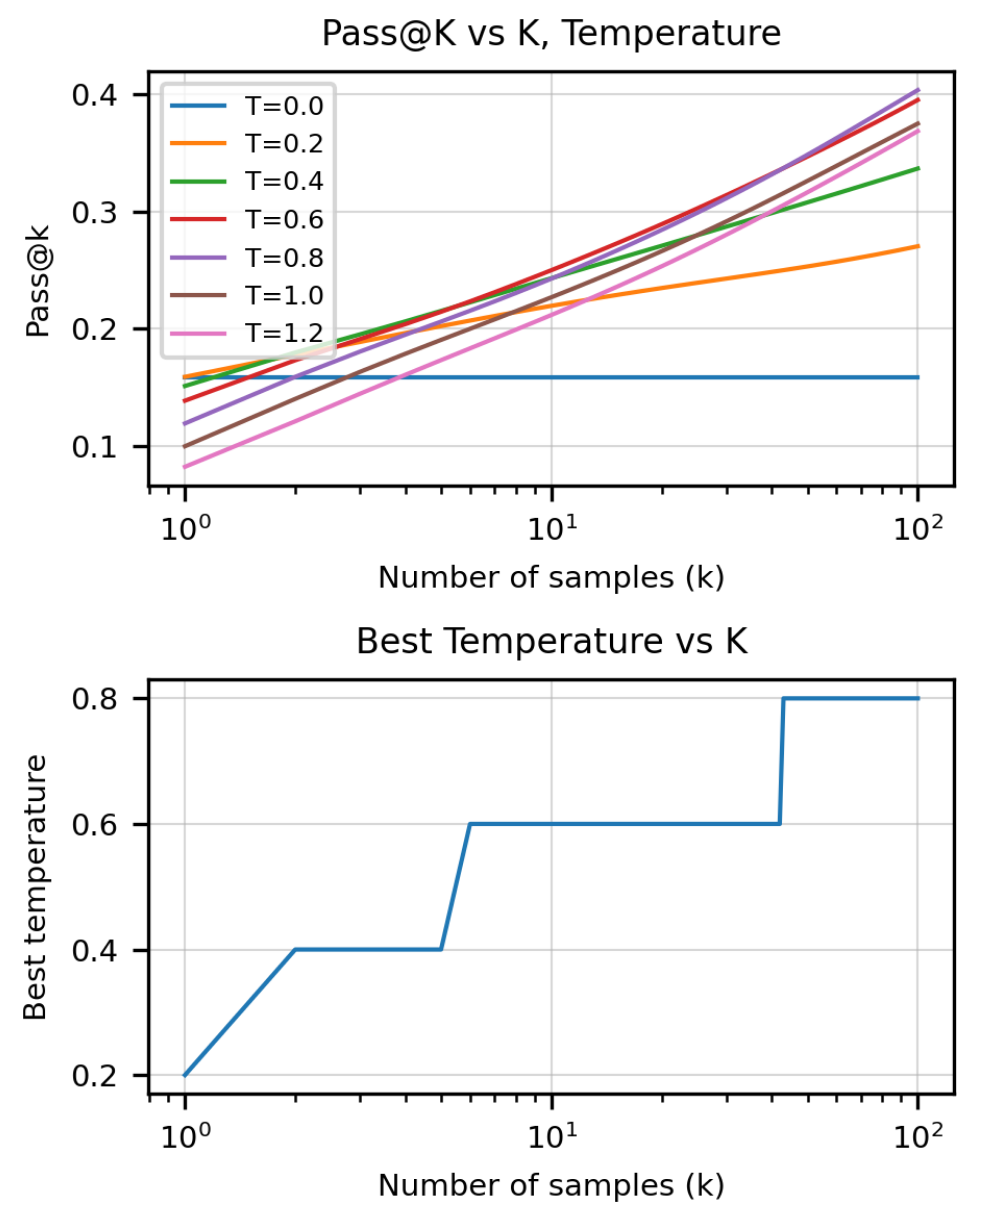
\includegraphics[width=0.5\linewidth]{PassVsK.png}
    \caption{Vergleich von $k$ aus der pass@k Metrik gegen die \texttt{temperature} des LLMs. Entnommen aus \cite{chenEvaluatingLargeLanguage2021}.}
    \label{fig:Pass vs K}
\end{figure}

\subsection{Weitere Konfigurationsparameter}\label{ch:Versuchsaufbau:Weitere Konfig}

Neben der Konfiguration des LLMs ist auch die generelle Konfiguration der Experiment-Durchläufe relevant. Zuerst gillt klar zu stellen, dass diese Arbeit nicht den Rahmen hat um eine hohe Menge an Experiment-Durchläufen durchzuführen. Aus diesem Grund ist die Menge an Durchläufen für 1 Code-Generierungslösung x 1 Benchmark $n=1$.

Aus dieser Restriktion folgt auch eine Konsequenz für die zu meldende Metrik. für $pass@k$ mit einem $k=1$ und einem $n=1$ kollabiert die gegebene Formel aus \todo{ref} zu einem einfachen $c/n$, also dem Durchschnitt. Daher werden die Ergebnisse in $avg@1$ gemeldet.

\subsubsection{Agentische Limits}

Agentische Systeme die in dieser Arbeit getestet werden können die Menge an erlaubten Schritten konfigurieren. Diese werden daher möglichst gleichmäßig konfiguriert. Dies bedeutet im Detail:

\begin{itemize}
    \item \textbf{CodeTeam} erlaubt die Konfiguration der kompletten Entwicklugnsrunden und der jeweiligen Schritte des Codes \& des Analyzers. \\ \todo{Schritte aus Arbeit übernehmen}
    \item \textbf{Terminus-2} erlaubt die Konfiguration der kompletten Schritte des Agenten. Da es sich hier um einen einzelnen Agenten handelt, wird die Schrittmenge auf $75$\todo{!} gesetzt.
\end{itemize}

\section{Durchführung und Abweichungen}\label{ch:Durchführung und Abweichungen}

Diese Sektion beschreibt den Prozess der Durchführung für die einzelnen Experimente.

\subsection{Vergleich Paper gegen Orchestrator}

Zunächst erfolgt die Durchführung mit der etabliert werden soll, inwiefern die Evaluierungs Plattform in ihren Ergebnissen von denen der Original-Paper abweicht.

\subsubsection{Self Collaboration}

Self Collaboration wird wie im Original Paper \cite{dongSelfCollaborationCodeGeneration2024} durchgeführt. Dies bedeutet die Evaluierung gegen den HumanEval Benchmark mit folgenden Hyperparametern:

\begin{itemize}
    \item \texttt{temperture = 0}
    \item \texttt{top\_p = 0.95}
    \item \texttt{max \_tokens = 512}
\end{itemize}

Das Original Paper nutze das Model \texttt{gpt-3.5-turbo-0301}. Dieses Modell wurde bereits vor Ende des Jahres 2024 eingestellt \cite{DeprecationsOpenAIAPI}. Es wurde daher die Entscheidung getroffen ein abweichendes Modell zu nutzen. Die Wahl viel hier auf \texttt{gpt-3.5-turbo-0613}. Es muss erwähnt werden dass dieses Modell vergleichsweise neuer ist, es kann davon ausgegangen werden dass es also leistungsfähiger ist.

Weitere Parameter, spezifisch für diesen Durchlauf sind wie folgt:

\begin{itemize}
    \item Maximum Runden zwischen Coder und Tester: 4
    \item Maximum Schritte für jeden Coder: 10
\end{itemize}

\section{Einordnung gegenüber publizierten Ergebnissen}\label{Einordnung gegenüber publizierten Ergebnissen}

Zunächst muss die Frage geklärt werden, welche Ergebnisse sich aus den Experimenten ergeben haben, die publizierte Ergebnisse nachstellen sollten. Daraus lässt sich später schlussfolgern ob die selbst gebaute Evaluierungs Plattform die gegebenen Ansätze so nutzt wie es die Authoren intendiert haben.

\subsection{Self Collaboration}

Wie bereits beschrieben, musste die lokale Ausführung leider auf ein neueres Modell ausweichen, da das originelle Modell nicht mehr verfügbar ist. Dennoch soll hier verglichen werden:

\begin{table}[H]
    \centering
    \caption{Vergleich Original Paper \& Evaluierungsplattform gegen HumanEval Benchmark}
    \label{tab:humaneval_comparison}
    \begin{tabular}{@{}lcc@{}}
        \toprule
        Ansatz & HumanEval & HumanEval-ET \\
        \midrule
        Original Paper & 74.4\% & 56.1\% \\
        Evaluierungs Plattform & 91.5\% & 79.3\% \\
        \bottomrule
    \end{tabular}
\end{table}

Ersichtlich ist, dass die lokale Implementierung in der Evaluierungs Plattform bessere Ergebnisse erzielt hat. Dies lässt sich durch die Nutzung eines anderen Modells erklären.

Unabhängig davon etabliert dies die Tatsache, dass die lokale Implementierung funktionsfähig ist. Ergebnisse sind in diesem Falle besser als die der originellen Publikation \cite{dongSelfCollaborationCodeGeneration2024}.

\section{Ergebnisse}\label{ch:Ergebnisse}



\section{Weitere Beobachtungen}\label{ch:Weitere Beobachtungen}

\todo[inline]{Falls relevant könnte man hier Randinformation mit aufnehmen, also Laufzeiten, Token Kosten, Iterationen (Harness), solche Sachen halt}

\section{Zusammenfassung}\label{ch:Zusammenfassung}


\controlquestions{
Im Kapitel „Experimente / Verifikation / Test / Validierung“ einer Abschlussarbeit wird überprüft, ob die entwickelte Lösung, das System oder das Konzept den Anforderungen genügt und die Forschungsfrage(n) beantwortet werden können. 
Dieses Kapitel ist zentral für die Beurteilung der Qualität, Aussagekraft und Belastbarkeit der Arbeitsergebnisse.
\begin{enumerate}
    \item Wurde direkt aus den Forschungsfragen (bzw. abgeleiteten Unterfragen, vgl.~Kapitel \ref{ch:Motivation und Problemdefinition}) und den Anforderungen bzw. Konzept (vgl.~Kapitel \ref{ch:Anforderungen und Konzept}) hergeleitet, warum ein Experiment nötig ist und was dieses nachweisen wird?
    \item Ist klar formuliert, was mit den Experimenten bzw. Tests überprüft oder validiert werden soll?
    \item Wurde das Experiment valide durchgeführt (mit ausführlicher Begründnung)? Z.~B.:
        \begin{itemize}
            \item mit verschiedenen Werten?
            \item mit ausreichenden Wiederholungen?
            \item in einer definierten, stabilen Umgebung?
            \item mit dokumentierten Parametern (Wiederholbarkeit/Reproducability)?
        \end{itemize}
    \item Sind gewählte Metriken, Messgrößen oder Bewertungskriterien nachvollziehbar und sinnvoll?
    \item Ist der Aufbau der Experimente methodisch korrekt und reproduzierbar dokumentiert?
    \item Wird das Vorgehen bei der Durchführung (z.\,B.~Testfälle, Abläufe) ausreichend detailliert beschrieben?
    \item Würde eine Wiederholung des Vorgehens zu ähnlichen Ergebnissen führen?
    \item Wurden Testdaten begründet ausgewählt oder erstellt – und sind diese ggf. dokumentiert/verfügbar?
    \item Werden die Ergebnisse verständlich, differenziert und strukturiert dargestellt (z.\,B.~mit Tabellen, Diagrammen, Text)?
    \item Sind die Ergebnisse vollständig dokumentiert – nicht nur die erfolgreichen, sondern auch unerwartete oder problematische?
    \item Sind die Messergebnisse mit geeigneten Methoden ausgewertet (z.\,B.~statistisch, vergleichend)?
    \item Gibt es einen Vergleich/Einordnung mit bestehenden Ansätzen, Referenzwerten oder einer Baseline?
    \item Wurde auf Reproduzierbarkeit und Generalisierbarkeit eingegangen?
    \item Beantworten die Ergebnisse die aufgestellten Forschungsfragen oder Zielsetzungen?
\end{enumerate}
}
